In recent years, there has been growing interest in data visualization technologies for human-assisted data analysis using systems such as Polaris~\cite{Stolte:2008} and Spotfire~\cite{Ahlberg:1996}. While computers can provide high-speed and high-volume data processing, humans have both the domain knowledge and the ability to process data in parallel by using their visual systems \cite{Cleveland.McGill1984,Mackinlay:1986}. 
%Humans also provide the definition of what is valuable in an analysis.
Systems that rely on \emph{both} the processing capability of computer systems and human feedback, are more effective in extracting useful knowledge from the large amounts of data being generated than either by itself.

\subsection{Interactivity}
Visualization systems are most effective when they are interactive, thereby allowing a user to explore data and connect it to their domain knowledge and sense of what is important without breaking cognitive flow. 
Exploration of data consists not only in creating visualizations, but also in creating and modifying domain-specific computations in the data model. 
During the analytic process, a user may discover that parts of the data are not yet suitable for analysis. 

Preparing this data for analysis often requires data preparation tools external to the visual analysis environment, which forces the user to break their cognitive flow, launch another tool and reprocess her data before returning to her analysis. 
Recent work~\cite{Morton:2012} found that the most effective systems allow users to define these calculations as part of the analytic interaction, enabling the user to stay in the flow of analysis.

We have observed that one of the most common such data preparation tasks users perform is parsing date strings into scalar date representations.
Examination of author calculations in a public repository using our
visualization system showed that there are about as many workbooks containing date parsing calculations ($3.3\%$) as there are
integer type conversions of any kind ($3.4\%$).
Streamlining this task is the focus of this paper.

\subsection{Scalar Dates}

The SQL-99 standard defines three temporal scalar types: \functionname{DATE}, \functionname{TIMESTAMP} and \functionname{TIME}, 
which can be further qualified as either \functionname{WITH} or \functionname{WITHOUT} \functionname{TIME ZONE} (the \functionname{WITHOUT} form being more common.) 
These types are typically implemented as fixed-point offsets from some epoch (\eg Julian Days.) 
This makes them compact to store using columnar compression techniques such as those in C-Store~\cite{Stonebraker:2005} and MonetDB/X100~\cite{Zukowski:2006}, 
and further allows some temporal operations to be implemented efficiently using simple arithmetic. 
Thus from the RDBMS perspective, representing dates in scalar form provides benefits for users, both in terms of analytic richness and query performance.

From an analytic perspective, date types are dimensional (\ie independent variables) and can be used as either \emph{categorical} (simply ordered) or \emph{quantitative} (ordered with a distance metric) fields.
Categorical dates have a natural hierarchy associated with them generated by calendar \emph{binning}, which is much easier to specify and compute with a scalar representation.
Figure \ref{fig:I1} shows an example of binned categorical dates in a year/quarter hierarchy using a bar chart.

\begin{figure}[ht]
\centering
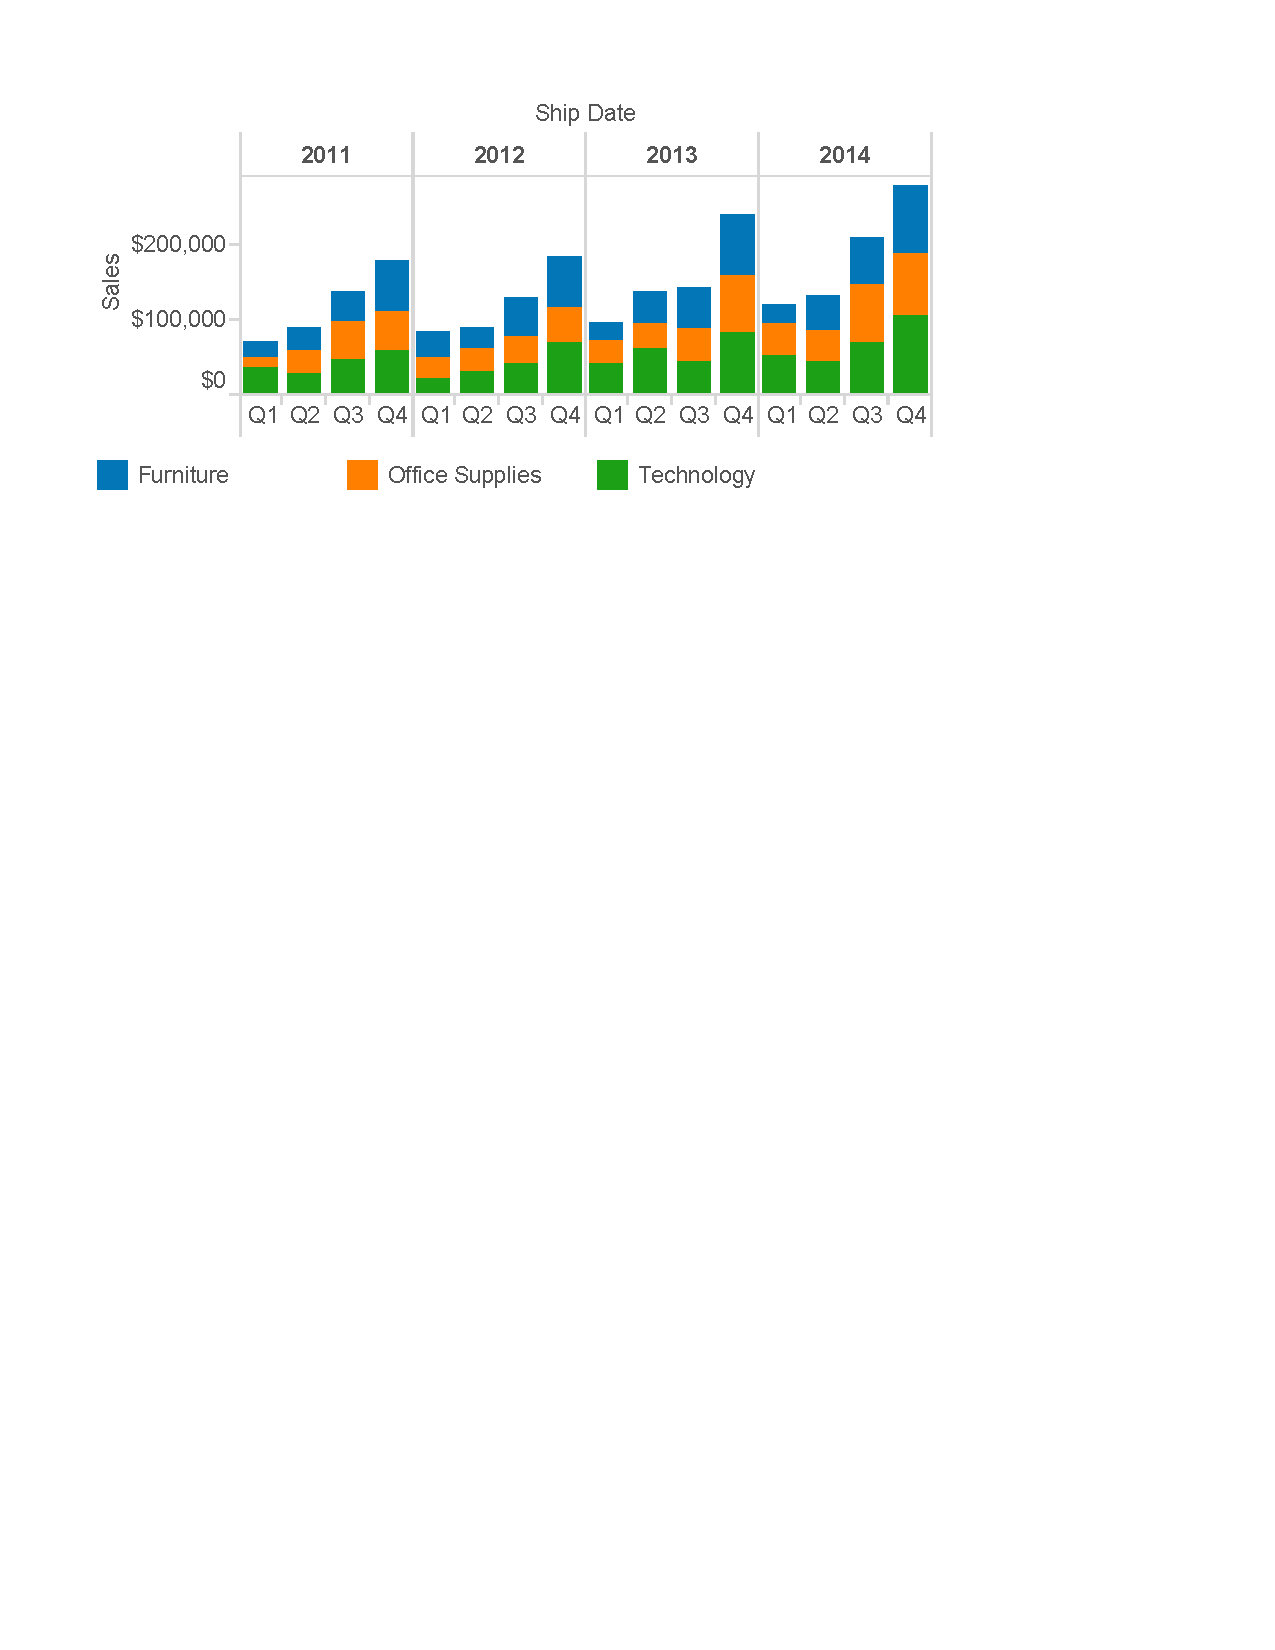
\includegraphics[width=\columnwidth]{figures/FigureI1}
\caption{Categorical Date Scalars.}
\label{fig:I1}
\end{figure}

Quantitative dates are typically used for time series on an axis that maps the underlying distance measure to display pixel distance. 
Figure \ref{fig:I2} shows the same sales data in a quantitative time series rolled up to the quarter level.

\begin{figure}[ht]
\centering
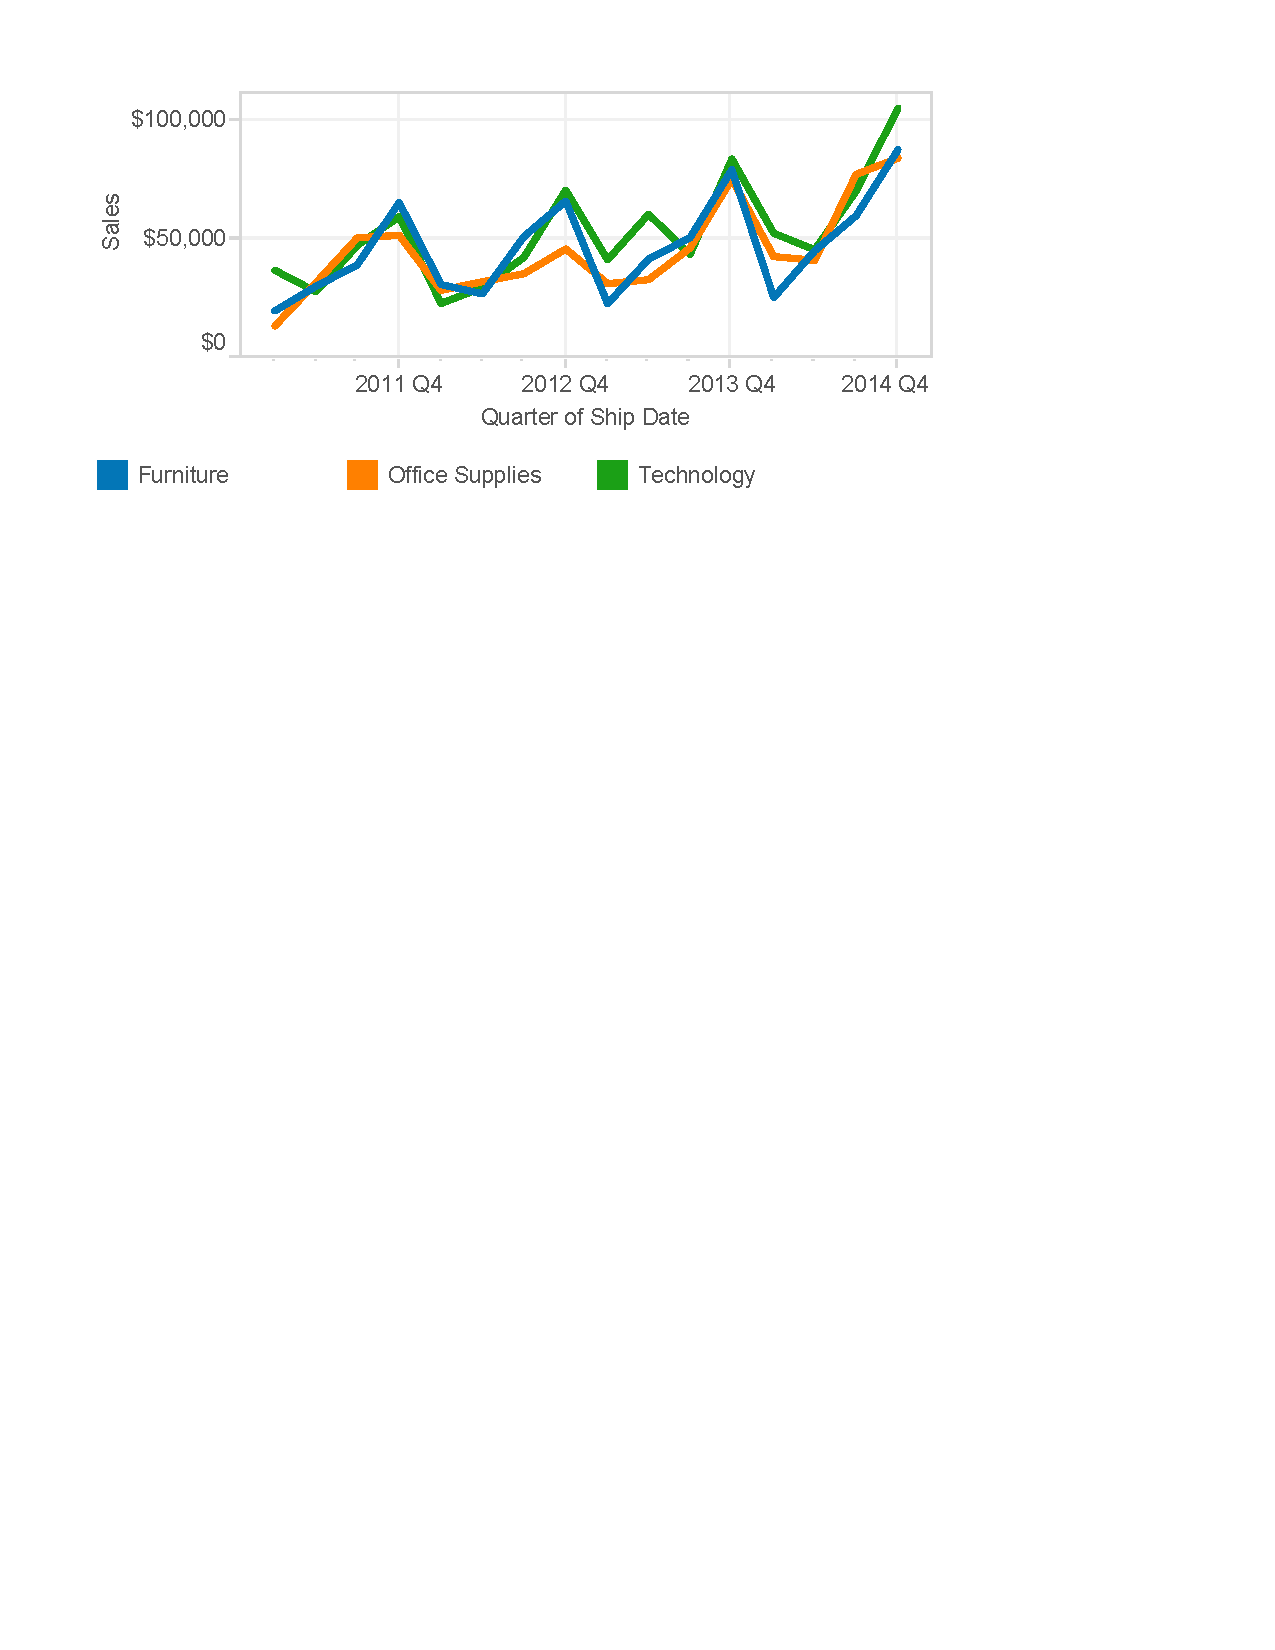
\includegraphics[width=\columnwidth]{figures/FigureI2}
\caption{Quantitative Date Scalars.}
\label{fig:I2}
\end{figure}

Both of these examples are much easier for users to specify and manipulate when the data is modeled by scalar dates.


\subsection{Parsing Dates}
A common form of the date parsing problem is converting columns of integers in the form \texttt{yyyyMMdd} to date scalars. \Naive\ users often solve this problem by converting the integer to a string and performing some locale-dependent string operations before casting the string back to a date, but this approach has a number of drawbacks. String operations are notoriously slow compared to scalar operations (typically 10-100x slower in modern RDBMSs). Default parsing of date formats is locale-dependent, and may not work when the parsing expression is shared across an international organization (\eg between the US and European offices). Such \textit{ad hoc} parsing code is often hard to understand and maintain because it uses a verbose, general-purpose string-handling syntax instead of a specialized domain language.

In Section~\ref{sec:experiments} we show that there are \emph{hundreds} of distinct temporal date formats in user data sets (Figure~\ref{fig:mdlerror}).
Some are common, but others can be quite idiosyncratic. 
Table~\ref{tab:dateformats} shows a selection of unusual date formats found in our corpus (the meanings of the ICU formatting codes can be found in Table~\ref{tab:icuformats}). 
The first example shows a time zone in the middle of the date and a year after the time; 
the second shows a leading unmatched bracket and a colon between the date and time components; 
the third shows confusion between the seconds' decimal point and the time part delimiter; 
the fourth shows a two digit year apostrophe on a four digit year and the fifth shows a dash separating the date and time components. 
This ``long tail'' of formats means that these idiosyncrasies are the rule, not the exception, 
so a small, fixed set of formats will not produce high reliability.

\begin{table}[ht]
\centering
\bgroup
\def\arraystretch{1.5}
\begin{tabular}{|p{0.4\linewidth}| p{0.4\linewidth}|}
\hline
\centering
\textbf{ICU Format} & \textbf{Example}\\ \hline
\scriptsize{EEE MMM dd HH:mm:ss zzz yyyy} & \scriptsize{Fri Apr 01 02:09:27 EDT 2011}\\ \hline
\scriptsize{[dd/MMM/yyyy:HH:mm:ss} & \scriptsize{[10/Aug/2014:09:30:40}\\ \hline
\scriptsize{dd-MMM-yy hh.mm.ss.SSSSSS a} & \scriptsize{01-OCT-13 01.09.00.000000 PM}\\ \hline
\scriptsize{MM ''yyyy} & \scriptsize{01 '2013}\\ \hline
\scriptsize{MM/dd/yyyy - HH:mm} & \scriptsize{04/09/2014 - 23:47}\\ \hline
\end{tabular}
\egroup
\caption{Unusual Date Formats.}
\label{tab:dateformats}
\end{table}

Several RDBMSs (\eg MySQL, Oracle and Postgres) provide row-level functions for parsing formatted dates, but a simple review of user attempts to use this functionality in published analyses showed a $15\%$ syntax error rate when using these functions unassisted. And even with perfect syntax, the user still has to interrupt her flow to learn a formatting syntax -- one that she will likely forget after this specific problem has been solved.

One approach might have been to design a graphical environment for constructing valid patterns and using visually compelling representations to reduce the cognitive load. 
But this approach provides no guarantee that the result would be correct if the user misunderstood the environment. 
Moreover, it only solves the syntax problem -- the user is still required to switch contexts.

Our solution was to develop two algorithms for automatically deriving the format string from the user's data with over $95\%$ parsing accuracy. Both algorithms are built based on classical machine learning algorithms that learn from pattern recognition to make data-driven predictions. We developed two algorithms because we were unaware of any previous work on this problem and we needed to be able to cross-validate our results on a large test corpus. With both approaches, the user can simply specify that the column is a date, and the visualization system can respond quickly and accurately enough to avoid interrupting the user's flow.

%\vidya{should this be its own section?}
%\richard{Ater discussion, we decide it was OK as is.}
\subsection{Related Work}
% vidya: this probably should be its own section
% hawkfish: Not sure it is big enough, but I can see the logic.

Data preparation has been considered an analytic bottleneck since at least the description of the Potter's Wheel system~\cite{Raman:2001}. Since then, several other interactive data preparation systems have been proposed, including Data Wrangler~\cite{Kandel:2011} and Google Refine~\cite{Refine}. While effective, these systems all make assumptions about possible date formats, which we suggest are too restrictive for real world data.

Various approaches have been described for deriving regular expressions, and a good overview is provided by Li et al. in their paper on the ReLIE system for deriving regular expressions given a starting expression provided by a domain expert~\cite{Li:2008}. The Minimum Descriptive Length technique first described in Rissanen~\cite{Rissanen:1978} was used in~\cite{Raman:2001} to generate regular expressions. 

There are several bodies of research on developing semantic parsers and grammars for interpreting time and date expressions. Lee \textit{et al} use a combinatory categorical grammar by combining the TIMEX3 standard~\cite{timex3} with contextual cues such as document creation time to determine the reference for parsing time expressions such as `2nd Friday of July'~\cite{LeeADZ14}.
 
\vidya{Should this be preceded by a bulleted list of contributions, under the section Contributions?}
%\subsection{Overview}
The rest of this paper is organized as follows: The next section introduces the parameters of the problem space. The following two sections describe the two different algorithms, one using Minimum Descriptive Length and the other using Natural Language Processing. In section 5, we evaluate the algorithms on a corpus of 30K columns, both by sampling the outputs manually and then by using the algorithms to validate each other. We then discuss future work in section 6 and conclude in section 7.


%\vidya{should this be its own section?}
\subsection{Contributions}

\begin{itemize}
\setlength\itemsep{0em}
\item By analyzing an online corpus, we provide evidence that practical date parsing requires the ability to recognize hundreds of formats;
\item We show how to extend prior work on Minimum Descriptive Length structure extraction to generate a freely available date format domain language with over 95\% accuracy;
\item We describe a second Natural Language Processing technique for generating the same date format domain language with similar accuracy. We describe how the basic algorithm is extended to support grammar variants and constraints unique to date formats. The parsing algorithm is extended to compute an overall dominant pattern over a data column;
\item We provide evidence that the development of multiple, independent parsing algorithms provides an effective means of cross-validation on large corpora;
\item We describe some limitations of this domain language that would improve its utility.
\end{itemize}
%% vidya: don't think we need this.
%% richard: It's kind of traditional in the DB community, but we can just leave it commented out - and put it back if they complain!
%\subsection{Organization}
%The rest of this paper is organized as follows: The next section provides background information for the problem space. The following two sections describe the two different algorithms, one using Minimum Descriptive Length and the other using Natural Language Processing. In section V, we evaluate the algorithms on a corpus of 30K columns, both by sampling the outputs manually and then by using the algorithms to validate each other. We then discuss related work in section VI, future work in section VII and conclude in section VIII.
